% !TEX root = IBL-InsolvabilityOfQuintic.tex
\chapter{Rings}
\label{chapter:Rings}
\thispagestyle{empty}
Our overarching goal, laid out in Chapter~\ref{chapter:PolyEquations}, is to show that there are quintic polynomials whose roots are \emph{not} expressible in terms of its coefficients using just the operations of addition, subtraction, multiplication, division, and the extraction of roots (thus implying that there is no ``quintic formula'' that is analogous to the quadratic formula). We decided that we would say that such polynomials are \emph{not} solvable by radicals, and in Chapter~\ref{chapter:SolvabilityByRadicals}, we finally were able to write down a formal definition of this term. We also proved there are many polynomials that are solvable by radicals. But, how do we show that a polynomial  is \emph{not} solvable by radicals? We start by taking a closer look at polynomials.


% % % % % % % % % % % % % % % % % % % % % % % % % % % % % % % % % % % % % % % % % % % %
% % % % % % % % % % % % % % % % % % % % % % % % % % % % % % % % % % % % % % % % % % % %
% SECTION
% % % % % % % % % % % % % % % % % % % % % % % % % % % % % % % % % % % % % % % % % % % %
% % % % % % % % % % % % % % % % % % % % % % % % % % % % % % % % % % % % % % % % % % % %
\section{Abstract rings}
As we investigate polynomials, it will be useful to harness (and abstract) the algebraic properties that they possesses. For example, if we add two polynomials in $\mathbb{Q}[x]$, we obtain a polynomial that is again in $\mathbb{Q}[x]$, and similarly for multiplication. Let's explore the structure of $F[x]$ in general (where $F$ is any field). 

\begin{definition}
Let $F$ be a field. The structure $(F[x],+,\cdot)$ consists of the set $F[x]$ together with the operations $+$ and $\cdot$ defined as follows. Let $p(x) = a_0 + a_1x + \cdots + a_mx^m$ and $q(x) = b_0 + b_1x + \cdots + b_nx^n$ with $m\le n$.
\begin{itemize}
\item \textbf{Addition:} $p(x) + q(x) =  (a_0 + b_0) + (a_1 + b_1)x + \cdots + (a_n + b_n)x^n$ (where $a_k = 0$ when $k> m$).
\item \textbf{Multiplication:} $p(x)\cdot q(x) = \displaystyle\sum_{k=0}^{m+n}c_kx^k$ where $c_k = a_0b_k + a_1b_{k-1} + \cdots + a_{k-1}b_1 + a_kb_0$.
\end{itemize}
We often refer to the entire structure $(F[x],+,\cdot)$ as simply $F[x]$.
\end{definition}

In the definition of polynomial multiplication above, $p(x)\cdot q(x)$ is just the result of applying the distributive law repeatedly to $(a_0 + a_1x + \cdots + a_mx^m)\cdot(b_0 + b_1x + \cdots + b_nx^n)$ and then grouping according to the powers of $x$. We will see that the operations of polynomial addition and multiplication have many familiar properties; let's prove a couple. 

\begin{problem}
Using the definitions of polynomial addition and multiplication  together with properties of fields, prove that for all fields $F$, both addition and multiplication in $F[x]$ are commutative.
\end{problem}

\begin{problem}
Let $F$ be any field. Find an additive identity for $F[x]$, and prove that it works. Also, if $p(x) = a_0 + a_1x + \cdots + a_mx^m$ is an arbitrary polynomial in  $F[x]$, find its additive inverse, and prove that it works.
\end{problem}

\begin{problem}
Which elements of $\mathbb{Q}[x]$ have a multiplicative inverse? Which do not? Justify your answer.
\end{problem}

As should be becoming clear, many of the properties of $F$ transfer to $F[x]$ (but not all!). Let's record some of those properties in a fact, which we will not prove. The existence of multiplicative inverses is notably absent.

\begin{fact}\label{fact.PolyRingAlgProperties}Let $F$ be any field. The following are true for $F[x]$.
\begin{itemize}
\item \textbf{Addition Laws:} Addition is associative and commutative. There is a unique additive identity, namely the constant zero polynomial, and every polynomial $p(x)$ has a unique additive inverse, denoted $-p(x)$.
\item \textbf{Multiplication Laws:} Multiplication is associative and commutative. There is a unique multiplicative identity, namely the constant polynomial $1$.
\item \textbf{Distributivity Laws:} For all $p(x),q(x),r(x) \in F[x]$, $p(x)(q(x)+r(x)) = p(x)q(x)+p(x)r(x)$ and $(q(x)+r(x))p(x) = q(x)p(x)+r(x)p(x)$.
\end{itemize}
\end{fact}

% % % % % % % % % % % % % % % % % % % % % % % % % % % % % % % % % % % % % % % % % % % %
% SUBSECTION
% % % % % % % % % % % % % % % % % % % % % % % % % % % % % % % % % % % % % % % % % % % %
\subsection{Definition and first examples}

Since $F[x]$ lacks multiplicative inverses for many of its elements, it does not form a field. Nevertheless, motivated by our desire to study polynomials, we will abstract the structure that is present so that we can prove theorems about polynomials over any field, instead of  working one field at a time. However, before we do, it's worth noting that there are many other structures that are not fields but do satisfy the laws in Fact~\ref{fact.PolyRingAlgProperties}---perhaps the most prominent one is the integers $\mathbb{Z}$. We  arrive at the definition of a ring.

\begin{definition}
A \textbf{ring} is a structure $(R,+,\cdot)$ consisting of a set $R$ together with two binary operations $+$ and $\cdot$ (which we call \emph{addition} and \emph{multiplication}) such that for some element $0\in R$ the following axioms hold.
\begin{itemize}
\item \textbf{Addition Axioms:} Addition is associative and commutative; the element $0$ is an additive identity; every  $x\in R$ has an additive inverse with respect to $0$, denoted $-x$.
\item \textbf{Multiplication Axioms:} Multiplication is associative.
\item \textbf{Distributivity Axioms:} For all $x,y,z \in R$, $x(y+z) = xy+xz$ and $(y+z)x = yx+zx$.
\end{itemize}
In the case that multiplication is commutative, $R$ is called a \textbf{commutative ring}, and in the case that there is a multiplicative identity, $R$ is called a \textbf{ring with unity} (or ring with $1$). 
\end{definition}

The notion of a ring is quite general, and the  terminology  ``commutative ring'' and ``ring with unity'' highlight some of the additional properties that $F[x]$ has, but arbitrary rings may not. But notice that fields have all of these properties \emph{and more}. The next definition  is meant to highlight this.

\begin{definition}
A \textbf{division ring} is a ring with unity such that every nonzero element has a multiplicative inverse.
\end{definition}

\begin{problem}
Fill in each box of the table below with \textbf{Y}es or \textbf{N}o. Assume that  $+$ and $\cdot$ are defined ``as usual'' for each set.\footnote{$2\mathbb{Z}$ denotes the even integers. The operations are usual integer addition and multiplication.}
\begin{flushleft}
\tabulinesep = 2mm
\begin{tabu}  {X[1.25,c,m]|[2pt]X[.8,c,m]|X[c,m]|X[c,m]|X[c,m]|X[.8,c,m]}
 & ring & commutative ring & ring with unity & division ring & field \\ \tabucline[2pt]{-}
$\mathbb{Z}$ &&&&& \\  \hline 
$2\mathbb{Z}$  &&&&& \\ \hline 
$\mathbb{N}$ &&&&& \\ \hline 
$\mathbb{Q}$ &&&&& \\ \hline 
$\mathbb{H}$ &&&&& \\ \hline 
$\mathbb{Z}_6$ &&&&& \\ \hline 
$\mathbb{R}[x]$ &&&&& \\ \hline 
$\left\{ a + bi\mid a,b\in \mathbb{Q}\right\}$ &&&&& \\ \hline 
$\left\{ a + bi\mid a,b\in \mathbb{Z}\right\}$ &&&&& \\ \hline 
\end{tabu}
\end{flushleft}
\end{problem}

% % % % % % % % % % % % % % % % % % % % % % % % % % % % % % % % % % % % % % % % % % % %
% SUBSECTION
% % % % % % % % % % % % % % % % % % % % % % % % % % % % % % % % % % % % % % % % % % % %
\subsection{Basic properties}

Many of the basic properties of fields hold also for rings, with essentially the same proofs, so we will just take them as fact.

\begin{fact}[Compare with Fact~\ref{thm.BasicFieldPropsUniqueness}]
Let $R$ be a ring. 
\begin{enumerate}
\item The additive identity is unique. If there exists a multiplicative identity, it is  unique.
\item Additive inverses are unique. If an element has a multiplicative inverse, it is unique.
\end{enumerate}
\end{fact}

\begin{fact}[Compare with Fact~\ref{thm.BasicFieldProps}]
Let $R$ be a ring. 
\begin{enumerate}
\item For all $x\in R$, $x\cdot0 = 0 = 0\cdot x$.
\item For all $x,y\in R$, $(-x)y = -(xy)$ and $x(-y) = -(xy)$.
\item If $R$ contains at least two elements and has a multiplicative identity, then the additive and multiplicative identities are different, i.e.~$0\neq 1$.
\end{enumerate}
\end{fact}

Let's explore one further property that fields possess but is not listed above: for all $x$ and $y$ in a field, if $xy = 0$, then $x=0$ or $y=0$. 

\begin{definition}
Let $R$ be a ring. An element $a\in R$ is called a \textbf{zero divisor} if $a$ is nonzero and there exists a nonzero $b\in R$ such that $ab=0$. A ring is called an  \textbf{integral domain} if it is a commutative ring with unity containing at least two elements but \emph{no zero divisors}.
\end{definition}

As remarked above, fields do not have zero divisors, so every field is indeed an integral domain. However, the prototypical integral domain (which explains the choice of name) is $\mathbb{Z}$. Let's look for others.

\begin{problem}
For each of the following rings, determine if there are zero divisors, and if so, find them all. Is the ring an integral domain?
\begin{multicols}{2}
\begin{enumerate}
\item $\mathbb{Z}_{5}$
\item $\mathbb{Z}_{10}$
\item $\mathbb{H}$
\item $\mathbb{R}[x]$
\end{enumerate}
\end{multicols}
\end{problem}

When working with integral domains, the following property is key.

\begin{theorem}[Cancellation Property]\label{thm.IntegralDomainCancel}
Let $R$ be an integral domain. For all $a,b,c\in R$, if $ab = ac$, then either $a=0$ or $b=c$. 
\end{theorem}

\begin{problem}
What properties of integral domains did you use in your proof of Theorem~\ref{thm.IntegralDomainCancel}? Can you rewrite the theorem to be more general? Try.  
\end{problem}

Let's pause to collect and organize all of our new definitions.

\begin{problem}
Complete the following Venn Diagram by adding in shapes for each of the following terms. Try to provide examples that live in each of the gaps, but we have not encountered enough examples (in these notes) to cover all gaps yet.
\begin{multicols}{3}
\begin{itemize}
\item Fields
\item Rings
\item Commutative Rings
\item Rings with unity
\item Division Rings
\item Integral domains
\end{itemize}
\end{multicols}
\begin{center}
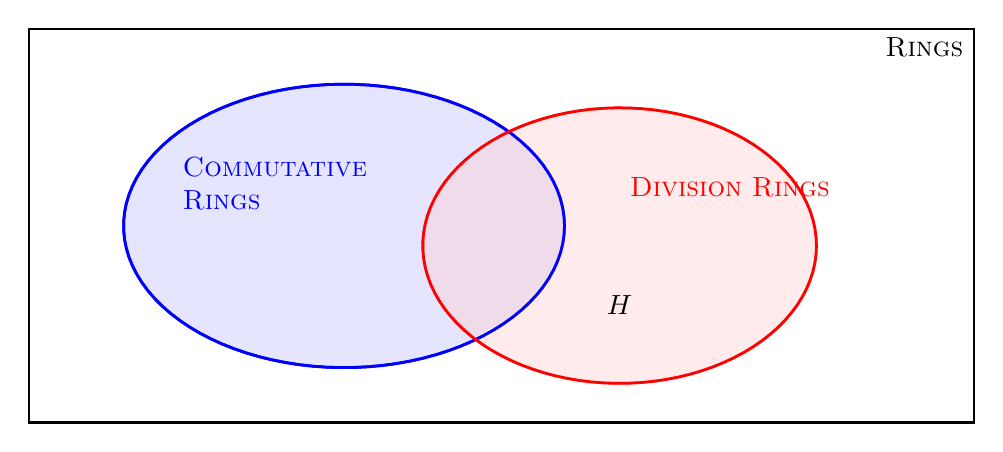
\begin{tikzpicture}[line width = 1]
\draw (0,0) rectangle (12,5);
\begin{scope}[shift={(4,2.5)}]
\fill[domain = 0:360,draw = blue, fill = blue!10, samples = 100] plot ({2.8*cos(\x)},{1.8*sin(\x)});
\end{scope}
\begin{scope}[shift={(7.5,2.25)}]
\fill[domain = 0:360,draw = red,fill = red!20, samples = 100,opacity=0.4] plot ({2.5*cos(\x)},{1.75*sin(\x)});
\end{scope}
\begin{scope}[shift={(4,2.5)}]
\draw[domain = 0:360,draw = blue, samples = 100,] plot ({2.8*cos(\x)},{1.8*sin(\x)});
\end{scope}
\begin{scope}[shift={(7.5,2.25)}]
\draw[domain = 0:360,draw = red, samples = 100] plot ({2.5*cos(\x)},{1.75*sin(\x)});
\end{scope}
\node[black, anchor = 20] at (12,5) {\textsc{Rings}};
\node[blue, anchor = 20, text width = 1in, align = flush left] at (4.5,3.5) {\textsc{Commutative Rings}};
\node[red, anchor = 20, text width = 1in, align = flush right] at (9.6,3.25) {\textsc{Division Rings}};
\node at (7.5,1.5) {$\mathbb{H}$};
\end{tikzpicture}
\end{center}
\end{problem}

% % % % % % % % % % % % % % % % % % % % % % % % % % % % % % % % % % % % % % % % % % % %
% SUBSECTION
% % % % % % % % % % % % % % % % % % % % % % % % % % % % % % % % % % % % % % % % % % % %
\subsection{Units}

Unless $R$ is actually a division ring, not all elements of $R$ will have a multiplicative inverse. Let's explore those elements that \emph{do} have an inverse.

\begin{definition}
Let $R$ be a ring with unity containing at least two elements. Then, $u\in R$ is called a \textbf{unit} if $u$ has a multiplicative inverse. The set of all units in $R$ is denoted $U(R)$.
\end{definition}


\begin{problem}
For each of the following rings, find all of the units, i.e.~determine $U(R)$.
\begin{multicols}{2}
\begin{enumerate}
\item $\mathbb{Z}$
\item $\mathbb{Z}_{5}$
\item $\mathbb{R}$
\item $\mathbb{R}[x]$
\end{enumerate}
\end{multicols}
\end{problem}

\begin{problem}
Consider the ring $\mathbb{Z}_{20}$. Find all units of $\mathbb{Z}_{20}$ and also find all zero divisors. What do you notice?
\end{problem}

\begin{problem}
Let $n$ be a positive integer. Make a conjecture about $U(\mathbb{Z}_n)$ by filling in the blank:  $U(\mathbb{Z}_n) = \{a\in \mathbb{Z}_n\mid\text{ \fillInBlank{fill in the blank} }\}$. What evidence do you have?
\end{problem}

\begin{theorem}\label{thm.UnitIsNotZeroDivisor}
Let $R$ be a ring with unity containing at least two elements. If $u\in R$ is a unit, then $u$ is \emph{not} a zero divisor.
\end{theorem}

\begin{problem}
Either prove or disprove the \emph{converse} of Theorem~\ref{thm.UnitIsNotZeroDivisor}.
\end{problem}

\begin{theorem}\label{thm.UnitsFormGroup}
Let $R$ be a ring with unity containing at least two elements. Then $(U(R),\cdot)$ is a group.
\end{theorem}


% % % % % % % % % % % % % % % % % % % % % % % % % % % % % % % % % % % % % % % % % % % %
% % % % % % % % % % % % % % % % % % % % % % % % % % % % % % % % % % % % % % % % % % % %
% SECTION
% % % % % % % % % % % % % % % % % % % % % % % % % % % % % % % % % % % % % % % % % % % %
% % % % % % % % % % % % % % % % % % % % % % % % % % % % % % % % % % % % % % % % % % % %
\section{An aside: matrix rings}

Matrix rings are really the prototypical ring with unity. Although you may have only seen matrices with real entries, it turns out that we can do matrix arithmetic with other types of entries, e.g.~entries from $\mathbb{C}$ or $\mathbb{Z}$. In fact, the usual matrix addition and multiplication makes sense when the entries come from any ring.

\begin{definition}
Let $R$ be a ring and $n$ a positive integer. Then $M_{n}(R)$ denotes the set of all $n\times n$ matrices whose entries come from $R$. The structure $(M_{n}(R),+,\cdot)$ consists of the set $M_{n}(R)$ of all $n\times n$ matrices whose entries come from $R$, together with the operations of usual matrix addition and matrix multiplication. 
\end{definition}

\begin{problem}
Provide examples of matrices satisfying each of the following conditions.
\begin{multicols}{2}
\begin{enumerate}
\item $A\in M_{3}(\mathbb{C})$ but $A\notin M_{3}(\mathbb{R})$
\item $B\in M_{2}(\mathbb{H})$ but $B\notin M_{2}(\mathbb{C})$
\item $C\in M_{2}\left(\mathbb{Q}\left(\sqrt{5}\right)\right)$ but $C\notin M_{2}(\mathbb{Q})$
\item $D\in M_{2}\left(\mathbb{R}[x]\right)$ but $D\notin M_{2}(\mathbb{R})$
\end{enumerate}
\end{multicols}
\end{problem}

\begin{problem}
Verify that $M_{2}(\mathbb{Z})$ is closed under matrix multiplication.
\end{problem}

The next fact shows that $M_{n}(R)$ is a ring with unity (for each positive $n$). Afterward, we will explore some of the other ring properties we discussed above.

\begin{fact} Let $R$ be any ring. The following are true for $M_{n}(R)$.
\begin{itemize}
\item \textbf{Addition Laws:} Addition is associative and commutative. There is a unique additive identity, namely the matrix with all entries equal to $0$, and every matrix $A$ has a unique additive inverse, denoted $-A$.
\item \textbf{Multiplication Laws:} Multiplication is associative. There is a unique multiplicative identity, namely the matrix with $1$'s on the main diagonal and $0$'s everywhere else.
\item \textbf{Distributivity Laws:} For all $A,B,C \in M_{n}(R)$, $A(B+C) = AB+AC$ and $(B+C)A = BA + CA$.
\end{itemize}
\end{fact}

\begin{problem}
Is $M_{2}(\mathbb{R})$ commutative? Prove your answer.
\end{problem}

\begin{problem}
Does $M_{2}(\mathbb{R})$ have zero divisors? Prove your answer. 
\end{problem}

The collection of units in a matrix ring forms a group with respect to matrix multiplication by Theorem~\ref{thm.UnitsFormGroup}. It is a very important object and even has a special name.

\begin{definition}
Let $R$ be a ring and $n$ a positive integer. The \textbf{general linear group} over the ring $R$,  denoted $\operatorname{GL}_n(R)$, is the group of units in the ring $M_{n}(R)$.
\end{definition}

\begin{problem}
Show that $\begin{bmatrix} i & 3\\ 0& i\end{bmatrix}\in\operatorname{GL}_{2}(\mathbb{C})$ by finding a multiplicative inverse for it. Also, find two different matrices in $M_{2}(\mathbb{C})$ that are \emph{not} in  $\operatorname{GL}_{2}(\mathbb{C})$.
\end{problem}


% % % % % % % % % % % % % % % % % % % % % % % % % % % % % % % % % % % % % % % % % % % %
% % % % % % % % % % % % % % % % % % % % % % % % % % % % % % % % % % % % % % % % % % % %
% SECTION
% % % % % % % % % % % % % % % % % % % % % % % % % % % % % % % % % % % % % % % % % % % %
% % % % % % % % % % % % % % % % % % % % % % % % % % % % % % % % % % % % % % % % % % % %
\section{Polynomial rings}
Our study of rings was motivated by our desire to learn more about polynomials, and we now dive a little deeper into the theory of polynomial rings. Ultimately, we will focus on polynomials rings $F[x]$ where $F$ is a field. In this section, we will see that $F[x]$ behaves in many ways like the integers $\mathbb{Z}$: $F[x]$ is an integral domain, there is a division algorithm for $F[x]$, there exists a greatest common divisor for polynomials, and there is a notion of primes and prime factorizations. 
Let's start with some important terminology.

\begin{definition}
Let $R$ be a ring, and let  $p(x)\in R[x]$ be a \emph{nonzero} polynomial. If $p(x) = a_0 + a_1x + \cdots + a_nx^n$ with $a_n \neq 0$, then $n$ is called the \textbf{degree} of $p(x)$, denoted $\deg p(x)$. In words, $\deg p(x)$ is the highest power of $x$ in $p(x)$ with a nonzero coefficient. The degree of the zero polynomial is undefined.
\end{definition}

\begin{problem}
Determine the degree of each of the following polynomials.
\begin{enumerate}
\item $q(x) = 4x^5 + 2x^2 + 5 -8x^2 +2x^5$ in the ring $\mathbb{Z}[x]$
\item $r(x) = 4x^5 + 2x^2 + 5 -14x^2 +2x^5$ in the ring $\mathbb{Z}_6[x]$
\item $p(t) = (3t^2-\sqrt{2})(-1 + 2t -t^3)$ in the ring $\mathbb{R}[t]$
\item $s(x) = (5-i)^8 - (5-s)^8$ in the ring $\mathbb{C}[s]$
\end{enumerate}
\end{problem}

The degree function is incredibly useful when working with polynomials---let's prove a couple of properties about it. 

\begin{theorem}\label{thm.DegreePolySum}
Let $R$ be a ring. If $p(x)$ and $q(x)$ are nonzero polynomials $R[x]$, then $\deg(p(x) + q(x)) \le \max(\deg p(x),\deg q(x))$ or  $\deg(p(x) + q(x))$ is undefined.
\end{theorem}

\begin{problem}
Give an example of polynomials $p(x),q(x)\in \mathbb{Q}[x]$ such that $\deg(p(x)+q(x)) < \max(\deg p(x),\deg q(x))$.
\end{problem}

\begin{theorem}\label{thm.DegreePolyProduct}
Let $D$ be an integral domain. If $p(x)$ and $q(x)$ are nonzero polynomials $D[x]$, then $\deg(p(x)q(x)) = \deg p(x) + \deg q(x)$, and in particular, $\deg(p(x)q(x))$ is defined.
\end{theorem}

\begin{problem}
Give an example of nonzero polynomials $p(x),q(x)\in \mathbb{Z}_{10}[x]$ such that $\deg(p(x)q(x)) \neq \deg p(x) + \deg q(x)$. Why does this not contradict Theorem~\ref{thm.DegreePolyProduct}?
\end{problem}

\begin{corollary}\label{cor.PolysOverIntegralDomains}
If $D$ is an integral domain, then $D[x]$ is an integral domain.
\end{corollary}

% % % % % % % % % % % % % % % % % % % % % % % % % % % % % % % % % % % % % % % % % % % %
% SUBSECTION
% % % % % % % % % % % % % % % % % % % % % % % % % % % % % % % % % % % % % % % % % % % %
\subsection{Division algorithm}
Here we explore what it means for one polynomial to divide another as well as the idea of a quotient and remainder for division. These should be familiar from previous classes for $\mathbb{R}[x]$, but here we see that they generalize to arbitrary $F[x]$ for $F$ a field.
 
\begin{definition}
Let $R$ be a ring, and let $a,b\in R$. We say that $b$ \textbf{divides} $a$ (or $b$ is a \textbf{divisor} of $a$) if there exists some $q\in R$ such that $a = bq$.
\end{definition}

\begin{problem}
Consider the polynomial $p(x) = x^2 - 1$ in $\mathbb{Q}[x]$.
\begin{enumerate}
\item Does $x+1$ divide $p(x)$ in $\mathbb{Q}[x]$? Why or why not?
\item Does $p(x)$ divide $x+1$ in $\mathbb{Q}[x]$? Why or why not?
\item Does $3$ divide $p(x)$ in $\mathbb{Q}[x]$? Why or why not?
\end{enumerate}
\end{problem}

\begin{theorem}\label{thm.LinearFactorOfPolyImpliesRoot}
Let $p(x)\in R[x]$ with $R$ a ring. If $c\in R$ and $(x-c)$ divides $p(x)$, then $p(c) = 0$.
\end{theorem}

Even if $b(x)$ does not divide $a(x)$, it can still be useful to perform the division to obtain a quotient and remainder.

\begin{problem}
Consider the polynomials $a(x) = x^4+x^3-8x +5$  and $b(x) = x^2 -3$ in $\mathbb{Q}[x]$. Use polynomial long division to show that $b(x)$ does not divide $a(x)$. What is the quotient and what is the remainder? Write $a(x)$ as $a(x) = b(x)q(x) + r(x)$ for some $q(x),r(x)\in \mathbb{Q}[x]$ with $\deg r(x) < \deg b(x)$.
\end{problem}

The ``division algorithm'' (Theorem~\ref{thm.DivisionAlgorithm}) formalizes what results from long division. And, it turns out that it is true for polynomials over any field (not just $\mathbb{Q}$). The next lemma prepares for the proof of the division algorithm. 

\begin{lemma}
Let $F$ be a field, and let $a(x),b(x)\in F[x]$ with $\deg a(x)\ge \deg b(x)$. Assume that $a(x) = a_0 + a_1x + \cdots + a_nx^n$ with $a_n\neq 0$ and $b(x) = b_0 + b_1x + \cdots + b_mx^m$ with $b_m\neq 0$. Set $a_1(x) =  a(x) - b(x)a_nb_m^{-1}x^{n-m}$. Then $\deg a_1(x) < \deg a(x)$, and $b(x)$ divides $a(x) - a_1(x)$.
\end{lemma}

Suppose we are trying to divide $b(x)$ into $a(x)$. How do we find the quotient and the remainder? Well, if the degree of $a(x)$ is smaller than the degree of $b(x)$ there is nothing to do (and if $a(x) = 0$, there is also nothing to do). Otherwise, we can use the previous lemma to produce a polynomial $a_1(x)$ such that $\deg a_1(x) < \deg a(x)$ and $b(x)$ divides $a(x) - a_1(x)$, or in other words, $a(x) - a_1(x) = b(x)q_1(x)$ for some $q_1(x)$. Now, suppose we repeat the process and divide $b(x)$ into the resulting $a_1(x)$ to produce $a_2(x)$ and $q_2(x)$. Continuing in this fashion, we produce $a_2, q_2, a_3,q_3 \ldots, a_k,q_k$, stopping once the degree of $a_k(x)$ becomes smaller than the degree of $b(x)$ (or $a_k(x)=0$). In total, we get something like the following.

\begin{align*}
a(x) - a_1(x) & = b(x)q_1(x)\\
a_1(x) - a_2(x) & = b(x)q_2(x)\\
a_2(x) - a_3(x) & = b(x)q_3(x)\\
& \;\;\vdots\\ 
a_{k-1}(x) - a_{k}(x) & = b(x)q_k(x)
\end{align*}
Adding the above equations together and moving things around, we arrive at  \[a(x) = b(x)\left(q_1(x) + q_2(x) + q_3(x) +\cdots + q_k(x)\right) + a_k(x)\]
with the degree of $a_k(x)$ being less than the degree of $b(x)$. Thus, $a_k(x)$  is the remainder and $q_1(x) +\cdots + q_k(x)$ the quotient. This is the rough idea behind the division algorithm.

\begin{theorem}[Division algorithm for {$F[x]$}]\label{thm.DivisionAlgorithm}
Let $F$ be a field, and let $a(x),b(x)\in F[x]$ with $b(x) \neq 0$. Then there exist $q(x),r(x)\in F[x]$ such that 
\[a(x) = b(x)q(x) + r(x)\]
with $\deg r(x) < \deg b(x)$ or $r(x) = 0$.
\end{theorem}

The division algorithm is the theoretical analogue of long division. If you want to divide concrete polynomials, use long division, but if you want to prove something about divisibility for arbitrary polynomials, use the division algorithm. It is often used to prove a polynomial $b(x)$ actually divides another polynomial $a(x)$. The strategy is to apply the division algorithm to produce the equation $a(x) = b(x)q(x) + r(x)$ (with $\deg r(x) < \deg b(x)$ or $r(x) = 0$) and then use this to show that, in fact, $r(x)=0$,  implying that $a(x) = b(x)q(x)$ as desired. Let's try using this approach to prove the converse of Theorem~\ref{thm.LinearFactorOfPolyImpliesRoot}.

\begin{theorem}\label{thm.RootImpliesLinearFactorOfPoly}
Let $p(x)\in F[x]$ for $F$ a field. If $c\in F$ and $p(c) = 0$, then $(x-c)$ divides $p(x)$.
\end{theorem}

\begin{problem}
Consider the polynomial  $p(x) = x^2+x+3$ in $\mathbb{Z}_5[x]$. Compute $p(c)$ for each $c\in \mathbb{Z}_5$, and use the results to determine which polynomials of the form $(x-c)$ divide $p(x)$. Factor $p(x)$ into a product of degree $1$ polynomials in $\mathbb{Z}_5[x]$, if possible.
\end{problem}

\begin{problem}
Consider the polynomial  $p(x) = x^2+x+1$ in $\mathbb{Z}_5[x]$. Explain why $p(x)$ cannot be factored into a product of degree $1$ polynomials in $\mathbb{Z}_5[x]$.
\end{problem}

% % % % % % % % % % % % % % % % % % % % % % % % % % % % % % % % % % % % % % % % % % % %
% SUBSECTION
% % % % % % % % % % % % % % % % % % % % % % % % % % % % % % % % % % % % % % % % % % % %
\subsection{Greatest common divisors}

The fact that there is a division algorithm for $F[x]$ (Theorem~\ref{thm.DivisionAlgorithm}) is a rather special property for a ring to possess, and it has several important consequences. The first one we'll explore is the existence of a ``greatest common divisor'' for two polynomials, and our first order of business is to try to decide on a reasonable definition of this.
 
\begin{problem}
What are the common divisors of $6$ and $-9$ in $\mathbb{Z}$? Which one is the greatest common divisor?
\end{problem}

\begin{problem}\label{prob.GCDExlore}
Consider the polynomials $a(x) = 2x^2-2$ and $b(x) = 2x^2+2x-4$ in $\mathbb{Q}[x]$.
\begin{enumerate}
\item Show that $x-1$ is a common divisor of $a(x)$ and $b(x)$ by finding  $q(x),s(x)\in \mathbb{Q}[x]$ such that $a(x) = (x-1)q(x)$ and $b(x) = (x-1)s(x)$.
\item Show that $-2(x-1)$ is a common divisor of $a(x)$ and $b(x)$ by finding  $q(x),s(x)\in \mathbb{Q}[x]$  such that $a(x) = -2(x-1)q(x)$ and $b(x) = -2(x-1)s(x)$.
\item Show that $100(x-1)$ is a common divisor of $a(x)$ and $b(x)$ by finding  $q(x),s(x)\in \mathbb{Q}[x]$ such that $a(x) = 100(x-1)q(x)$ and $b(x) = 100(x-1)s(x)$.
\end{enumerate}
Which one, if any, would be a good choice as the ``greatest common divisor''?
\end{problem}

The previous problem highlights that there are several (actually, infinitely many) choices for the ``greatest common divisor'' of two polynomials. Our choice for which one we call the greatest common divisor is, in some sense, the simplest one.

\begin{definition}
A polynomial $p(x)$ of degree $n$ is called \textbf{monic} if the coefficient of $x^n$ (i.e.~the leading coefficient) is $1$.
\end{definition}

For example, $7-2x+x^2$ is monic, since the coefficient of $x^2$ is $1$. However, neither $7-2x+3x^2$ nor $7-2x-x^2$ are monic.

\begin{definition}
Let $F$ be a field, and let $a(x), b(x)\in F[x]$ be nonzero polynomials. A polynomial $d(x)\in F[x]$ is called a \textbf{greatest common divisor} of $a(x)$ and $b(x)$ if
\begin{enumerate}
\item $d(x)$ is monic,
\item $d(x)$ divides both $a(x)$ and $b(x)$,
\item if $h(x)$ divides both $a(x)$ and $b(x)$, then $h(x)$ divides $d(x)$.
\end{enumerate}
\end{definition}

Thus, in Problem~\ref{prob.GCDExlore},  the greatest common divisor of the polynomials $a(x)$ and $b(x)$ is $x-1$.
That said, we don't yet know that a greatest common divisor always exists, but let's start by showing that if one exists, there is only one.

\begin{lemma}\label{lem.GCDUnique}
Let $F$ be a field, and let $a(x), b(x)\in F[x]$ be nonzero polynomials. If $d_1(x)$ and $d_2(x)$ are  greatest common divisors of $a(x)$ and $b(x)$, then $d_1(x)=d_2(x)$.
\end{lemma}

We now work towards the existence of a greatest common divisor for arbitrary polynomials in $F[x]$ (for arbitrary fields). The proof of this result is tightly tied to analyzing certain combinations of the polynomials $a(x)$ and $b(x)$. Let's explore this a bit.

\begin{problem}\label{prob.GCDIdeal}
Consider the polynomials $a(x) = 2x^2-2$ and $b(x) = 2x^2+2x-4$ in $\mathbb{Q}[x]$.  Define \[I = \{f(x)a(x) + g(x)b(x)\mid f(x),g(x)\in \mathbb{Q}[x]\}.\]
\begin{enumerate}
\item Write down 5 different polynomials that are in the set $I$. 
\item Show that $x-1$ divides an arbitrary polynomial in $I$.
\end{enumerate}
\end{problem}

The idea behind the second part of Problem~\ref{prob.GCDIdeal} can be used to prove the following general result about sets like $I$.

\begin{theorem}\label{thm.HalfOfGCDProof}
Let $F$ be a field, and let $a(x), b(x)\in F[x]$ be nonzero polynomials. Define \[I = \{f(x)a(x) + g(x)b(x)\mid f(x),g(x)\in F[x]\}.\]
If $h(x)$ divides both $a(x)$ and $b(x)$, then $h(x)$ divides every $c(x)\in I$.
\end{theorem}

The existence and uniqueness of greatest common divisors in $F[x]$ is presented in the following fact.

\begin{fact}\label{fact.GCD}
Let $F$ be a field, and let $a(x), b(x)\in F[x]$ be nonzero polynomials. There exists a unique greatest common divisor of $a(x)$ and $b(x)$, and if $d(x)$ is the greatest common divisor, then \[d(x) = f(x)a(x) + g(x)b(x),\]
for some $f(x),g(x)\in F[x]$.
\end{fact}

The proof of this fact is interesting, but let's content ourselves to just outline it. The approach is fairly straight forward. Define \[I = \{f(x)a(x) + g(x)b(x)\mid f(x),g(x)\in F[x]\}.\]  Theorem~\ref{thm.HalfOfGCDProof} tells us that every common divisor of $a(x)$ and $b(x)$ is a divisor of every polynomial in $I$. Thus, if $I$ contains a monic, common divisor of $a(x)$ and $b(x)$, it must be the greatest common divisor. So, we look for a common divisor of $a(x)$ and $b(x)$ in $I$. And to do this, the key idea is to choose a polynomial of smallest degree in $I$.

Let $m$ be the smallest degree of all nonzero polynomials in $I$  (which exists by the Well-Ordering Property of the natural numbers). Choosing any polynomial of degree $m$ in $I$, we can divide out the leading coefficient to get a \emph{monic} polynomial $d(x)$, which we can show is still in $I$. The polynomial $d(x)$ will be the greatest common divisor.

To see that $d(x)$ divides $a(x)$, we use Theorem~\ref{thm.DivisionAlgorithm} (the division algorithm) to write $a(x) = d(x)q(x) + r(x)$ for $q(x),r(x)\in F[x]$ with $\deg r(x) < \deg d(x)$ or $r(x) = 0$. Towards a contradiction, assume $r(x) \neq 0$. Now, since $d(x)\in I$, there exist $f_d(x),g_d(x)\in F[x]$ such that
\begin{align*}
r(x) & = a(x) - d(x)q(x)\\
& = a(x) - [f_d(x)a(x) + g_d(x)b(x)]q(x)\\
& = [1-f_d(x)q(x)]a(x) + [-g_d(x)q(x)]b(x)\\
&\in I.
\end{align*}
Since $\deg r(x) < \deg d(x)$, this contradicts the fact that $d(x)$ had the smallest possible degree of all polynomials in $I$. Thus, $r(x) = 0$, and $d(x)$ divides $a(x)$. A similar argument shows that $d(x)$ also divides $b(x)$, so $d(x)$ is a monic, common divisor of $a(x)$ and $b(x)$. And, Theorem~\ref{thm.HalfOfGCDProof} shows that $d(x)$ is a greatest common divisor. But then, it is the unique greatest common divisor by Lemma~\ref{lem.GCDUnique}.

Using Fact~\ref{fact.GCD}, we can rewrite the set $I$ is a very nice way.

\begin{corollary}
Let $F$ be a field, and let $a(x), b(x)\in F[x]$ be nonzero polynomials. Define \[I = \{f(x)a(x) + g(x)b(x)\mid f(x),g(x)\in F[x]\}.\]
If $d(x)$ is the greatest common divisor of $a(x)$ and $b(x)$, then $I = \{p(x)d(x)\mid p(x)\in F[x]\}$.
\end{corollary}

With similar ideas as in the proof of Fact~\ref{fact.GCD}, one can prove the following fact that characterizes the greatest common divisor in several different ways.

\begin{fact}
Let $F$ be a field, and let $a(x), b(x)\in F[x]$ be nonzero polynomials. Define \[I = \{f(x)a(x) + g(x)b(x)\mid f(x),g(x)\in F[x]\}.\]
For any polynomial $d(x)\in F[x]$, the following are equivalent:
\begin{enumerate}
\item $d(x)$ is the greatest common divisor of $a(x)$ and $b(x)$;
\item $d(x)$ is a monic common divisor of $a(x)$ and $b(x)$, and $d(x) \in I$;
\item $d(x)$ is a monic, and $I = \{p(x)d(x)\mid p(x)\in F[x]\}$.
\end{enumerate}
\end{fact}

So, you may be wondering: how do we compute the greatest common divisor of two polynomials? First think about how you would compute the greatest common divisor of $168$ and $180$. Really, think about it\ldots Many people will factor both  $168$ and $180$ into primes and then multiply the prime factors they have in common. This works for integers, and in fact, it will also work for polynomials once we develop the notion of a ``prime polynomial.'' However, there is another approach, which in general is way more efficient: the Euclidean Algorithm. We will not develop it here, but you are encouraged to look it up (perhaps starting on \href{https://en.wikipedia.org/wiki/Polynomial_greatest_common_divisor}{Wikipedia}).

% % % % % % % % % % % % % % % % % % % % % % % % % % % % % % % % % % % % % % % % % % % %
% SUBSECTION
% % % % % % % % % % % % % % % % % % % % % % % % % % % % % % % % % % % % % % % % % % % %
\subsection{Irreducible polynomials}
We now develop the analogous notion of a prime number for polynomials, which will be \emph{irreducibility}.  The concept of irreducibility makes sense quite generally, so we start by defining it for any integral domain. Recall that, by Corollary~\ref{cor.PolysOverIntegralDomains}, $F[x]$ is always an integral domain when $F$ is a field. 

To motivate the definition, think about how prime integers are defined: $p\in \mathbb{Z}$ is prime if (1) $p>1$ and (2) $p=ab$ implies that $a=\pm 1$ or $b=\pm1$. Since the  units of $\mathbb{Z}$ are precisely $\pm1$, the second condition could be rewritten as ``$p=ab$ implies that $a$ or $b$ is a unit.'' Also, since we don't  want $1$ (or $-1$) to be considered prime, the first condition is mostly captured by ensuring that ``$p$ is not zero and not a unit.'' 

\begin{definition}\label{def.reducible}
Let $D$ be an integral domain. An element $p\in D$ is \textbf{irreducible} if 
\begin{itemize}
\item $p\neq 0$ and $p\notin U(D)$, and
\item for all $a,b\in D$, $p = ab$ implies $a\in U(D)$ or $b\in U(D)$.
\end{itemize} 
The element $p$ is \textbf{reducible} if it is not irreducible; that is if $p=0$, $p\in U(D)$, or there exist $a,b\in D$ such that $p = ab$ and $a,b\notin U(D)$. 
\end{definition}

\begin{problem}
Use Definition~\ref{def.reducible} to show that a field has no irreducible elements.
\end{problem}

\begin{problem}
What are the irreducible elements in $\mathbb{Z}$?
\end{problem}

In order to investigate irreducibility in an integral domain $D$, we need to know its units. Our overarching goal is to better understand polynomials, so let's 
start there. 

\begin{theorem}\label{thm.UnitsFAdjoinx}
Let $F$ be a field. Then $p(x)$ is a unit in $F(x)$ if and only if $\deg p(x) = 0$. 
\end{theorem}

Let's  rewrite our definition of reducibility in a more useable form for polynomials.
\begin{theorem}
Let $F$ be a field, and let $p(x)$ be a nonzero polynomial in $F[x]$. Then $p(x)$ is reducible if and only if $\deg p(x) > 0$ and there exist polynomials $a(x),b(x) \in F[x]$ such that $p(x) = a(x)b(x)$ with $\deg a(x) <\deg p(x)$ and $\deg b(x) <\deg p(x)$.
\end{theorem}

\begin{problem}
Determine if $p(x)$ is reducible or irreducible in the given ring. If it's reducible, write down a factorization.
\begin{multicols}{2}
\begin{enumerate}
\item $p(x) = x^2+1$ in $\mathbb{C}[x]$
\item $p(x) = x^2+1$ in $\mathbb{Q}[x]$
\item $p(x) = x^2+1$ in $\mathbb{Z}_2[x]$
\item $p(x) = x^2+1$ in $\mathbb{Z}_3[x]$
\end{enumerate}
\end{multicols}
\end{problem}

Let's catalog a couple of general irreducibility/reducibility results for polynomials of small degree.

\begin{theorem}
Let $F$ be a field. If $\deg p(x) = 1$, then $p(x)$ is irreducible.
\end{theorem}

\begin{theorem}\label{thm.ReducibilityTestDegree2or3}
Let $F$ be a field. If $\deg p(x) = 2,3$, then $p(x)$ is reducible if and only if $p(x)$ has a root in $F$.
\end{theorem}

\begin{problem}
Determine if $p(x)$ is reducible or irreducible in the given ring. If it's reducible, write down a factorization.
\begin{multicols}{2}
\begin{enumerate}
\item $p(x) = x^3-2$ in $\mathbb{Q}[x]$
\item $p(x) = x^3-2$ in $\mathbb{Z}_5[x]$
\end{enumerate}
\end{multicols}
\end{problem}

\begin{problem}
Determine if each of the following polynomials are reducible or irreducible in the given ring.
\begin{multicols}{2}
\begin{enumerate}
\item $p(x) = x^3-8$ in $\mathbb{Q}[x]$
\item $p(x) = x^3-8$ in $\mathbb{Z}_5[x]$
\item $r(x) = x^4-8x^2+15$ in $\mathbb{Q}$
\item $r(x) = x^4-8x^2+15$ in $\mathbb{Z}_5[x]$
\end{enumerate}
\end{multicols}
\end{problem}

To solidify the analogy between irreducible elements and primes, let's prove a factorization theorem.

\begin{theorem}\label{thm.FactorIrreducibles}
If $F$ is a field, then any polynomial of positive degree in $F[x]$ can be written as a product of polynomials that are irreducible in $F[x]$.
\end{theorem}

As you know, in the integers every number greater than or equal to $2$ can be factored into a product of primes in a way that is \emph{unique up to reordering the factors}. There is a similar uniqueness result for polynomials: any polynomial of positive degree in $F[x]$ can be written as a product of irreducible polynomials in a way that is unique up to reordering the factors and multiplying each factor by a unit.

\begin{problem}
Let $p(x) = 6 x^4 - 7 x^3 + 15 x^2 - 21 x - 9$. Then the following are two different factorizations of $p(x)$ into irreducibles in $\mathbb{Q}[x]$:
\begin{itemize}
\item $p(x) = (2x-3)(3x+1)(x^2+3)$, and
\item $p(x) = (x+\frac{1}{3})(2x^2+6)(3x-\frac{9}{2})$.
\end{itemize}
 Explain why the factorizations are the ``same'' up to reordering the factors and multiplying each factor by a unit.
\end{problem}

% % % % % % % % % % % % % % % % % % % % % % % % % % % % % % % % % % % % % % % % % % % %
% % % % % % % % % % % % % % % % % % % % % % % % % % % % % % % % % % % % % % % % % % % %
% SECTION
% % % % % % % % % % % % % % % % % % % % % % % % % % % % % % % % % % % % % % % % % % % %
% % % % % % % % % % % % % % % % % % % % % % % % % % % % % % % % % % % % % % % % % % % %
\section{Subrings and ideals}
We now return to general ring theory. As with groups and fields, the notion of a subring is fundamental. 

\begin{definition}
Let $(R,+,\cdot)$ be a ring, and let $S$ be a subset of $R$. Then $S$ is a \textbf{subring} of $R$ if $S$ is a ring in its own right with respect to operations $+$ and $\cdot$ \emph{inherited from $R$}.
\end{definition}

\begin{theorem}
Let $R$ be a ring, and let $S\subseteq R$. Then $S$ is a subring of $R$ if and only if 
\begin{enumerate}
\item $S$ is nonempty;
\item for all $x,y\in S$, $x+y\in S$ and  $xy\in S$; and
\item for all $x\in S$, $-x\in S$.
\end{enumerate}
\end{theorem}


